\chapter[SCP-075]{
    SCP-075 \\
    SCP-075
}

\label{chap:SCP-075}

\begin{figure}[H]
    \centering
    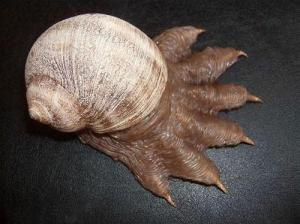
\includegraphics[width=0.5\linewidth]{images/SCP.075.jpg}
    \caption*{SCP-075。拍摄自\hyperref[chap:]{山田武博士}。}
\end{figure}

\bb{项目编号:}SCP-075

\bb{项目等级:}Euclid

\bb{特殊收容措施:}SCP-075应被收容于一个安全等级4的1 m x 1 m x 1 m抗腐蚀保险箱之中,这个保险箱亦应被保存于一个有着同样抗腐蚀处理的安全房间之中。在该房间之中的绝对湿度任何时候都不能超过1\%。医药用干燥剂应在任何时候都可以进行使用来保证该湿度。如果在075收容房间之中的湿度曾经达到1\%以上,所有人员都应马上撤离,并且该站点会被封锁直到湿度重新降到可接受范围。

所有进入075收容房间的人员都应穿着4级的聚丙烯(MOPP)防护服。注射测试,还有任何需要用到液体溶液的测试,都是被严格禁止的。如果任何溶液与075进行了接触,该区域将马上被封锁并且被干燥剂所填充,直到湿度重新进入可接受范围。严禁所有仍滞留在该区域之中的人员撤离。

\bb{描述:}SCP-075是一只长20cm,宽13cm,高15cm的大型蜗牛,它有着强健的、由6条有爪的触手所构成的伪足。075异乎寻常地重,有大约860kg的重量,这是一个我们现在还不能理解的特质。保持环境干燥是现在唯一已知能够收容075的手段,因为在一个几乎完全干燥的环境之中,075将会进入休眠状态。

当环境不再干燥时,075将会以与其质量和体型不相符的高速进行移动。它表现出了捕食者的行为,跳向它的猎物并且向它的猎物喷淋从它的伪足上的小孔之中分泌而出的高腐蚀性液体。这些分泌物比任何一种人类已知的物质的腐蚀性都要强。因为075在激活后的攻击性行为,这种化合物无法被收集。现今为止仍未找到一种可以完全抵御这种液体腐蚀的材料。

\bb{附录075-F:}想要收集075分泌物的尝试必须经过所有当时驻扎于站点之中的等级4人员批准,并且要在他们的监督下进行。但是上述人员的批准不能推翻严禁将任何溶液带到075身边的标准规则,这包括075的分泌物。

\bb{附录075-G:}一杯075的分泌物已经成功地通过使用\hyperref[chap:SCP-294]{SCP-294}进行了收集,现在正在测试是否有任何材料,能够免疫它的腐蚀。关于为什么\hyperref[chap:SCP-294]{SCP-294}给出的杯子能够免疫这些分泌物的腐蚀的测试也正在进行之中。
